\documentclass[12pt,english,fleqn]{extarticle}

\usepackage{geometry}
\geometry{verbose,tmargin=2.0cm,bmargin=2.0cm,lmargin=2.0cm,rmargin=2.0cm}
\setlength{\parskip}{\smallskipamount}
\setlength{\parindent}{0pt}

\usepackage{tikz}

\begin{document}

Contoh draw:

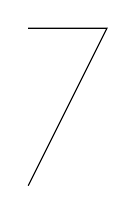
\begin{tikzpicture}
\path[draw] (0cm,0cm) -- (1cm,2cm) -- (0cm,2cm);
\end{tikzpicture}

Contoh fill:


\begin{tikzpicture}
\path[fill] (0cm,0cm) -- (1cm,2cm) -- (0cm,2cm);
\end{tikzpicture}


Contoh fill dan draw:


\begin{tikzpicture}
\path[fill=yellow,draw=red] (0cm,0cm) -- (1cm,2cm) -- (0cm,2cm);
\end{tikzpicture}


Contoh node:

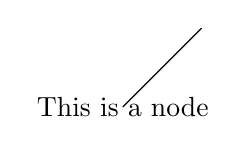
\begin{tikzpicture}
\draw (1cm,1cm) node {This is a node} -- (2cm,2cm);
\end{tikzpicture}


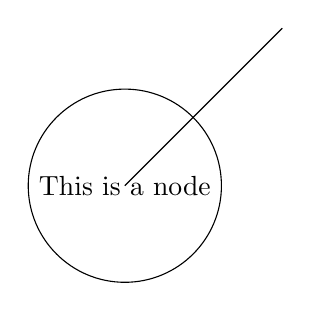
\begin{tikzpicture}
\draw (0cm,0cm) node[draw,circle] {This is a node} -- (2cm,2cm);
\end{tikzpicture}


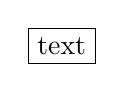
\begin{tikzpicture}
\draw (1,1) node[rectangle,draw] {text};
\end{tikzpicture}



\end{document}
